\section{Introduction}

% Abstract.
%
% Accurate automatic optimization heuristics are necessary for dealing with the complexity and diversity of modern hardware and software. Machine learning is a proven technique for learning such heuristics, but its success is bound by the quality of the features used. These features must be handcrafted by developers through a combination of expert domain knowledge and trial and error. This makes the quality of the final model directly dependent on the skill and available time of the system architect.
%
% Our work introduces a better way for building heuristics. We develop a deep neural network that learns heuristics over raw code, entirely without using code features. The neural network simultaneously constructs appropriate representations of the code and learns how best to optimize, removing the need for manual feature creation. Further, we show that our neural nets can transfer learning from one optimization problem to another, improving the accuracy of new models, without the help of human experts.
%
% We compare the effectiveness of our automatically generated heuristics against ones with features hand-picked by experts. We examine two challenging tasks: predicting optimal mapping for heterogeneous parallelism and GPU thread coarsening factors. In 89\% of the cases, the quality of our fully automatic heuristics matches or surpasses that of state-of-the-art predictive models using hand-crafted features, providing on average 14\% and 12\% more performance with no human effort expended on designing features.

There are countless scenarios during the compilation and execution of a program where decisions must be made as to how, or if, a particular optimisation should be applied. Modern compilers and runtimes are rife with hand-coded \emph{heuristics} which perform this decision making. The performance of programs is thus dependent on the quality of these heuristics.

handwritten heuristics require expert knowledge, take a lot of time to construct, and in many cases lead to sub-optimal decisions. Researchers have focused on machine learning as a means of constructing high-quality heuristics that often outperform their handcrafted equivalents~\cite{Micolet2016,Falch2015,Stephenson2005,Agakov,Cummins2016a}. A \emph{predictive model} is trained, using supervised machine learning, on empirical performance data and important quantifiable properties, or \emph{features}, of representative programs. The model learns the correlation between these features and the optimisation decision that maximises performance. The learned correlations are used to predict the best optimisation decisions for new programs. Previous works in this area were able to build machine learning based heuristics with less effort, that outperform ones created manually by experts~\cite{Grewe2013,Magni2014}.

Still, experts are not completely removed from the design process, which is shown in Figure~\ref{fig:overview-a}. Selecting the appropriate features is a manual undertaking which requires a deep understanding of the system. The designer essentially decides which compile or runtime characteristics affect optimisation decisions and expresses them in ways that make it easy to model their relationship to performance. Failing to identify an important feature has a negative effect on the resulting heuristic. One such feature was identified in Section~\ref{subsec:eval-extended}, causing performance to be 40\% lower on average.

To make heuristic construction fast and cheap, humans must be taken out of the loop. While techniques for automatic feature generation from the compiler IR have been proposed in the past~\cite{Namolaru2010a,Leather2014}, they do not solve the problem in a practical way. They are deeply embedded into the compiler, require expert knowledge to guide the generation, have to be repeated from scratch for every new heuristic, and their search time can be prohibitive. Inspired by the astounding success of recurrent neural networks at generating program code for benchmarking and compiler testing, I hypothesised that should a learning system should be able to automatically extract features from source code. The experiments showed that even this was a conservative target: with deep neural networks, one can bypass static feature extraction and learn optimisation heuristics directly on raw code.

\begin{figure}[t!]
	\centering
	\subfloat[Current state-of-practice]{%
		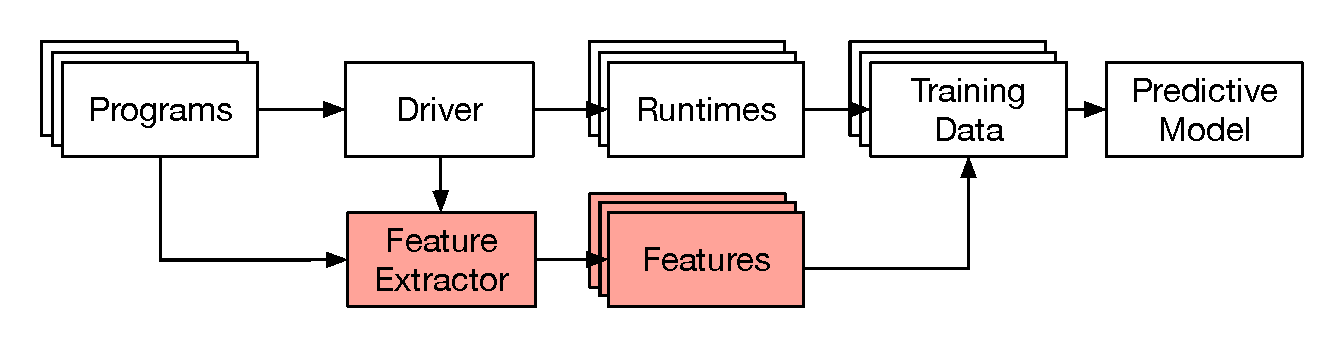
\includegraphics[width=.95\columnwidth]{img/training_model_a}%
		\label{fig:overview-a}%
	}\\*%
	\subfloat[The proposed approach]{%
		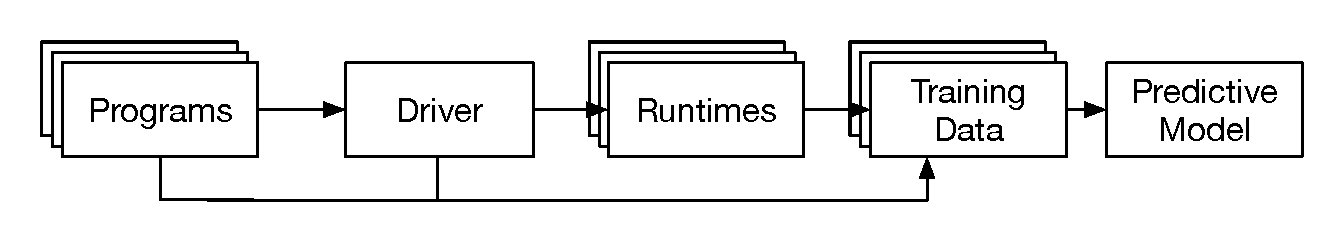
\includegraphics[width=.95\columnwidth]{img/training_model_b}%
		\label{fig:overview-b}%
	}%
	\caption[Using machine learning for compiler optimisations]{%
		Building a predictive model. The model is originally trained on performance data and features extracted from the source code and the runtime behaviour. The proposed approach bypasses feature extraction, instead learning directly over raw program source code.%
	}%
	\label{fig:overview}
\end{figure}

Figure~\ref{fig:overview-b} shows the proposed methodology. Instead of manually extracting features from input programs to generate training data, program code is used directly in the training data. Programs are fed through a series of neural networks which learn how code correlates with performance. Internally and without prior knowledge, the networks construct complex abstractions of the input program characteristics and correlations between those abstractions and performance. This chapter proposes replacing the need for compile-time or static code features, merging feature and heuristic construction into a single process of joint learning. The system admits auxiliary features to describe information unavailable at compile time, such as the sizes of runtime input parameters. Beyond these optional inclusions, the system is able to learn optimisation heuristics without human guidance.

By employing \emph{transfer learning}~\cite{Yosinski2014}, the proposed approach is able to produce high-quality heuristics even when learning on a small number of programs. The properties of the raw code that are abstracted by the beginning layers of our neural networks are mostly independent of the optimisation problem. Parts of the network may be reused across heuristics, and, in the process, can speed up learning considerably.

The approach is evaluated on two parallel compilation problems: heterogeneous device mapping and GPU thread coarsening. Good heuristics for these two problems are important for extracting performance from heterogeneous systems, and the fact that machine learning has been used before for heuristic construction for these problems allows direct comparison. Prior machine learning approaches resulted in good heuristics which extracted 73\% and 79\% of the available performance respectively but required extensive human effort to select the appropriate features. Nevertheless, the approach presented in this chapter was able to outperform them by 14\% and 12\%, which indicates a better identification of important program characteristics, without any expert help.

This chapter is organised as follows: Section~\ref{sec:deeptune} describes DeepTune, a novel system for building optimisation heuristics. In Sections~\ref{sec:deeptune-case-study-a} and~\ref{sec:deeptune-case-study-b}, case studies are presented, evaluating DeepTune's capabilities first at predicting heterogeneous device mapping, then thread coarsening. Section~\ref{sec:deeptune-transfer-learning} explores the novel transfer of information between the two problems. Then Section~\ref{sec:deeptune-internal-states} illuminates the inner workings of DeepTune. Finally, Section~\ref{sec:deeptune-conclusion} contains concluding remarks.
